\documentclass[a4paper, 11pt, titlepage]{article}

\usepackage{graphicx}
\usepackage{amssymb}
\usepackage{subfig}
\usepackage{amsmath}

\begin{document}
\title{Crisis Response in Social Networks}
\author{Joseph F. Harrison \\
        Matthew Revelle \\
        CSS 692, Social Network Analysis \\
        George Mason University}
\date{May 2010}
\maketitle

\tableofcontents
\newpage

\section{Introduction}

\begin{figure}[h]
\centering
\label{fig:all_tweets_over_time}
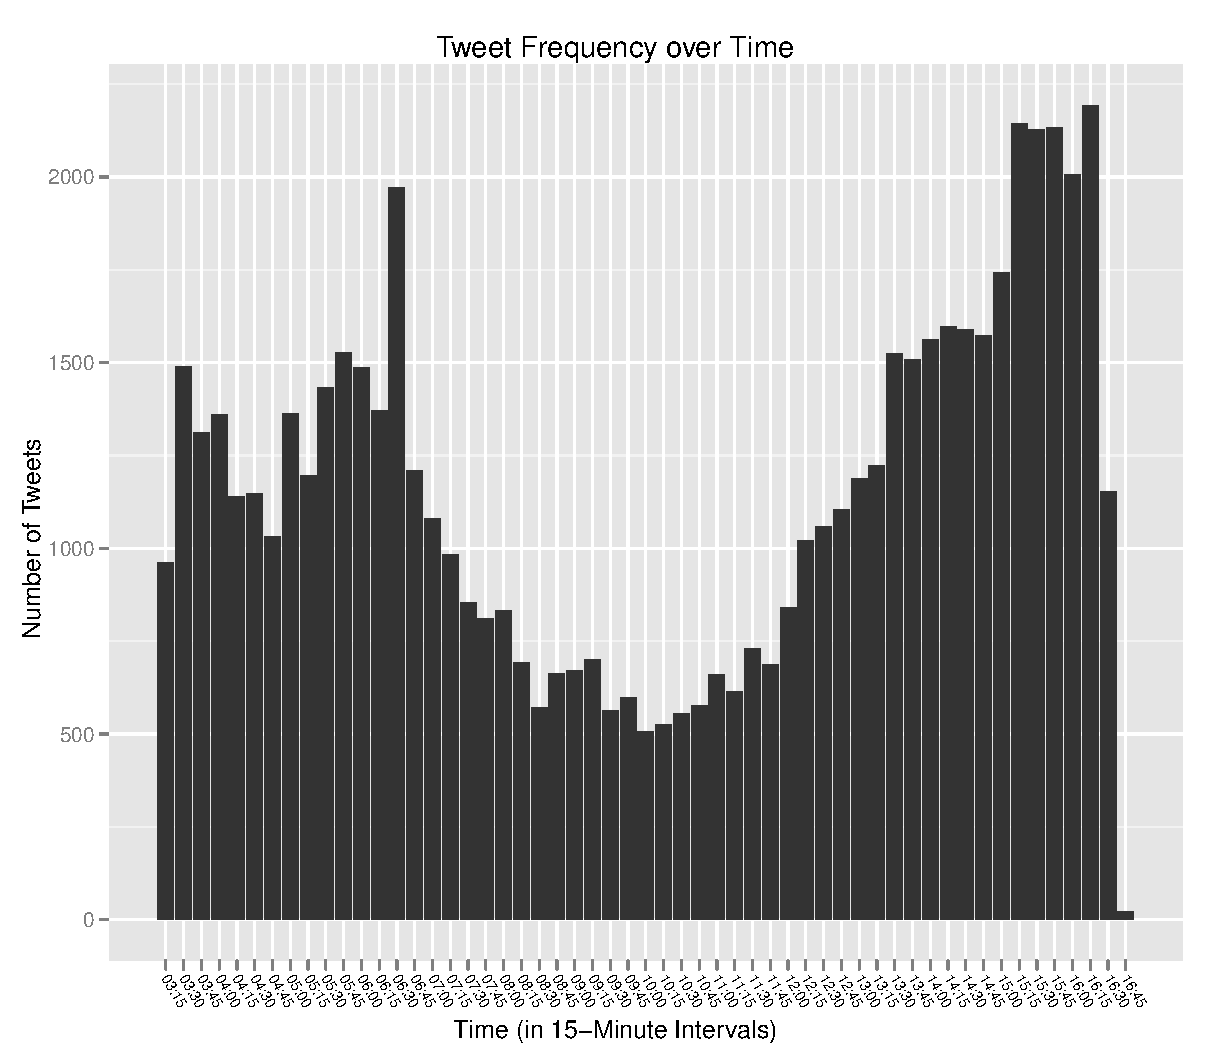
\includegraphics[width=120mm]{../figures/all_tweets_over_time}
\caption{All tweets over time..}
\end{figure}

\begin{figure}[h]
\centering
\label{fig:all_tweets_by_users}
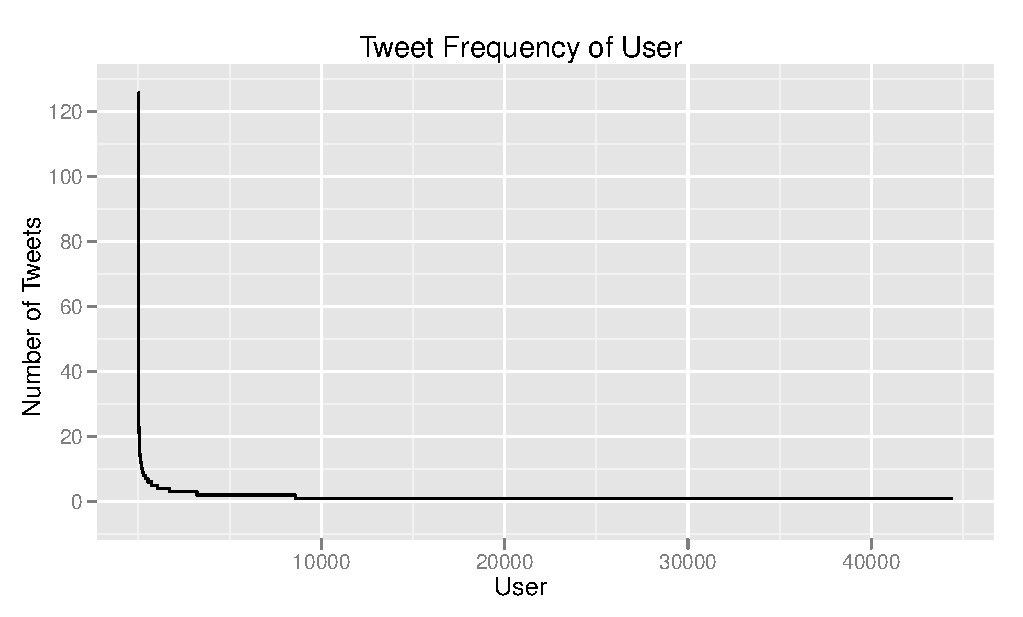
\includegraphics[width=120mm]{../figures/all_tweets_by_users}
\caption{All tweets over time..}
\end{figure}

\section{Retweets}

\begin{figure}[h]
\centering
\label{fig:rt_compare_over_time}
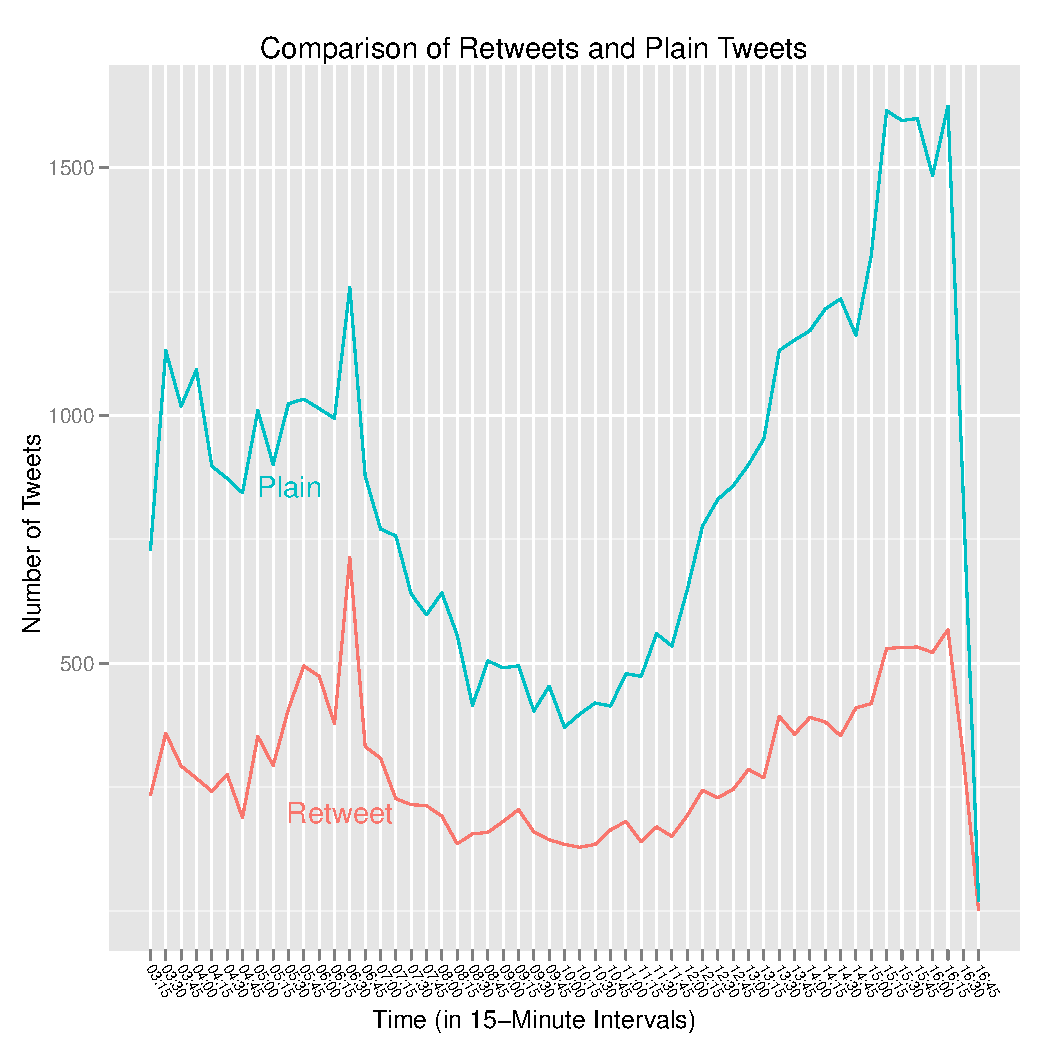
\includegraphics[width=120mm]{../figures/rt_compare_over_time}
\caption{Frequency of retweets compared to plain tweets over time.}
\end{figure}

\begin{figure}[h]
\centering
\label{fig:rt_top_50}
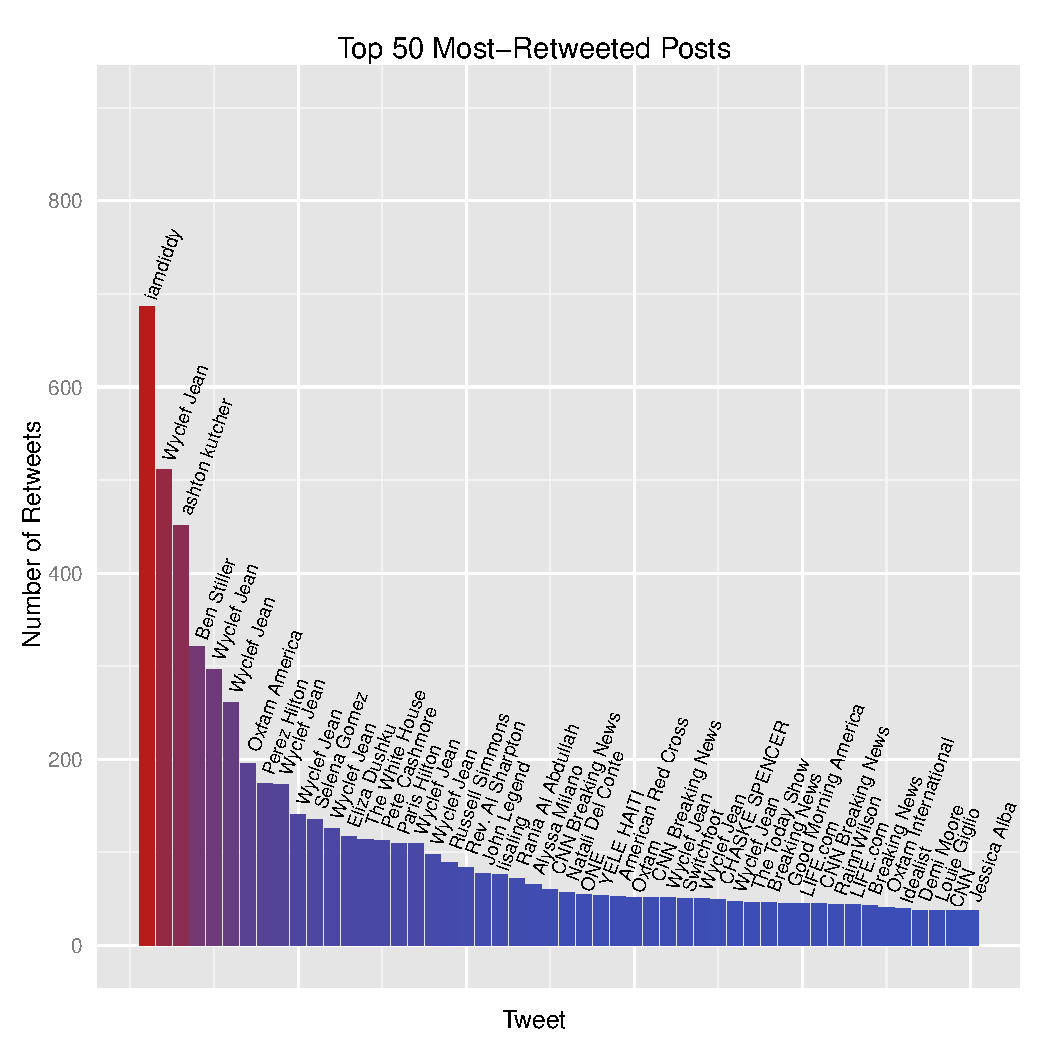
\includegraphics[width=120mm]{../figures/rt_top_50}
\caption{Top 50 most-retweeted posts.}
\end{figure}

\begin{figure}[h]
\centering
\label{fig:rt_top_10}
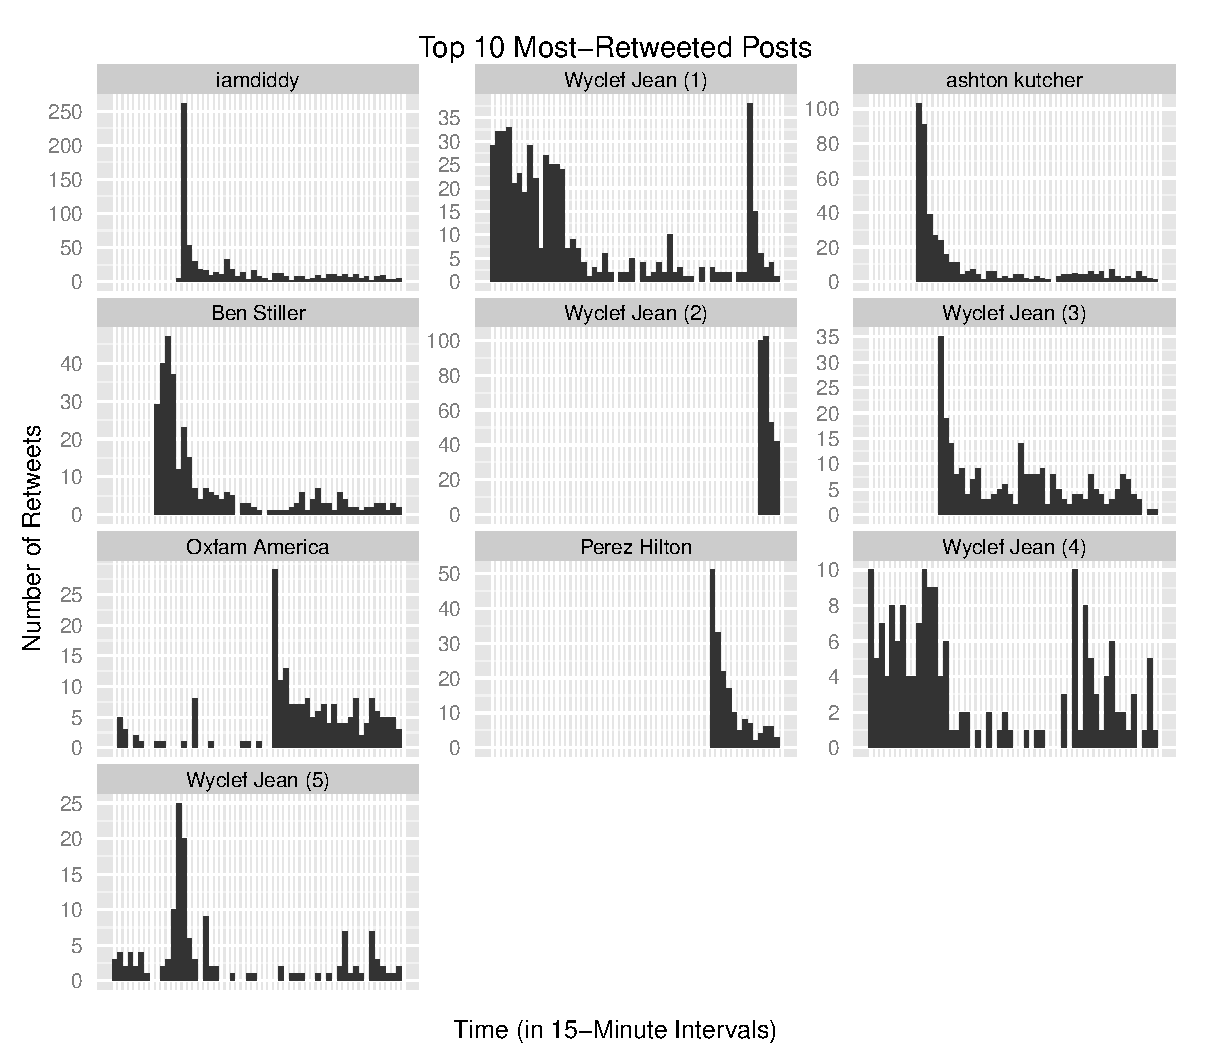
\includegraphics[width=120mm]{../figures/rt_top_10_over_time_free_scale}
\caption{Top 10 most-retweeted messages over time.}
\end{figure}

\begin{figure}[h]
\centering
\label{fig:rt_net_core}
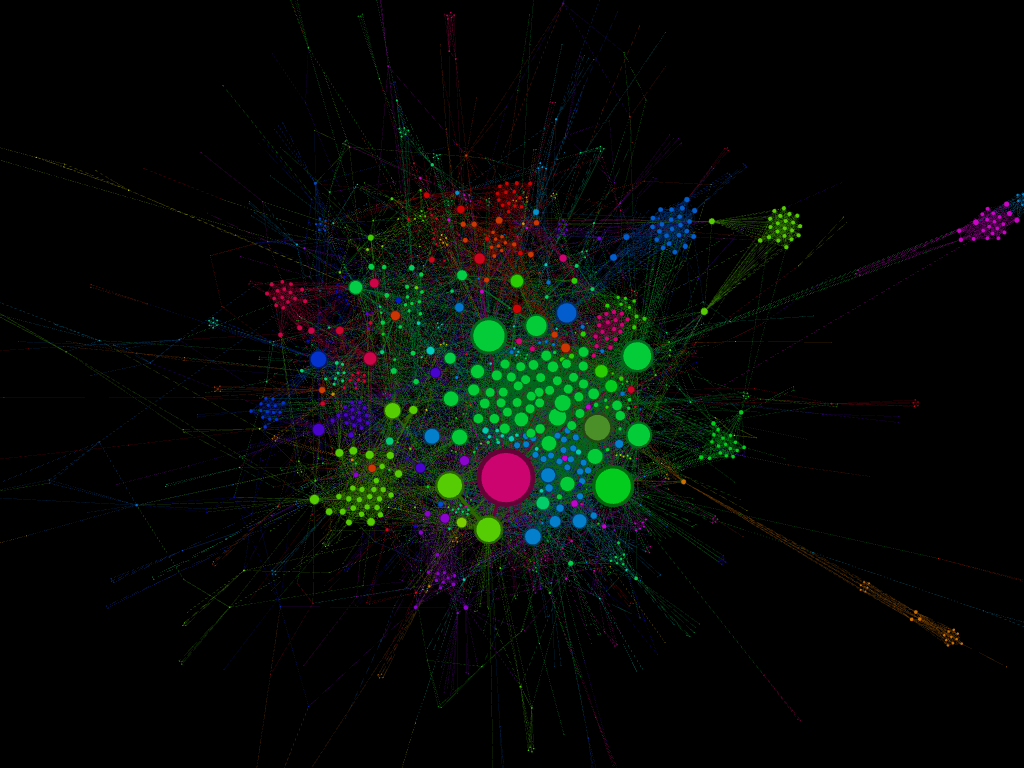
\includegraphics[width=120mm]{../figures/rt_net_core}
\caption{The core of the retweet network.}
\end{figure}

\begin{figure}[h]
\centering
\label{fig:rt_net_top_50}
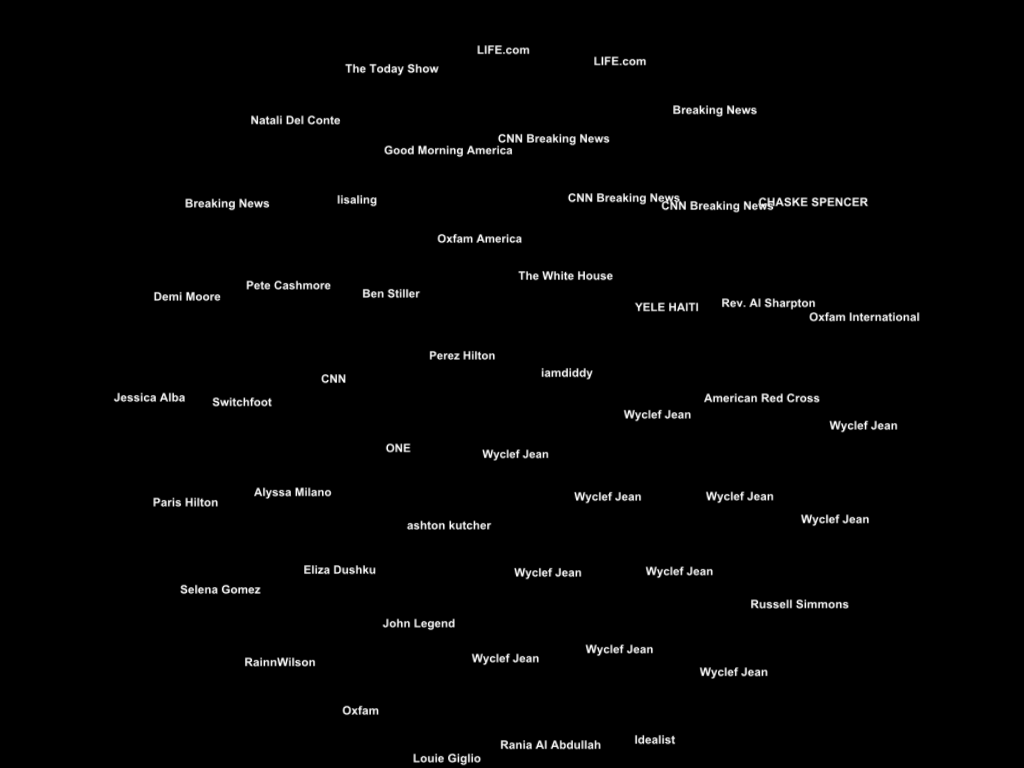
\includegraphics[width=120mm]{../figures/rt_net_top_50_tweets}
\caption{Top 50 most-retweeted posts in the network.}
\end{figure}

\begin{figure}[h]
\centering
\label{fig:rt_net_core_clusters}
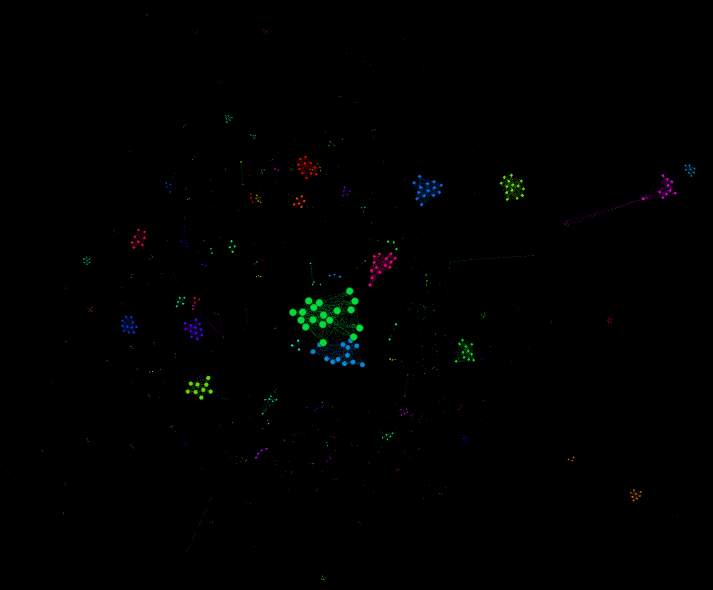
\includegraphics[width=120mm]{../figures/rt_net_core_clusters}
\caption{Clusters in the network core.}
\end{figure}

\begin{figure}[h]
\centering
\label{fig:rt_net_travel}
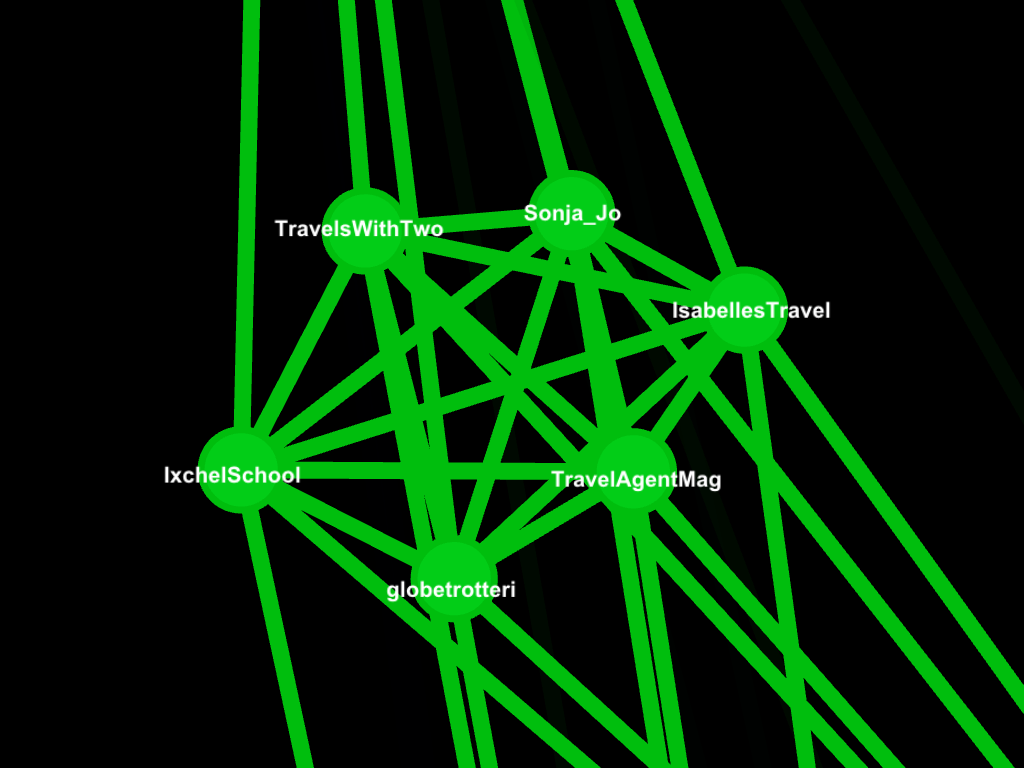
\includegraphics[width=120mm]{../figures/rt_net_travel}
\caption{A cluster of tweets from authors in the travel industry.}
\end{figure}

\begin{figure}[h]
\centering
\label{fig:rt_net_photos}
\subfloat[Two Clusters]{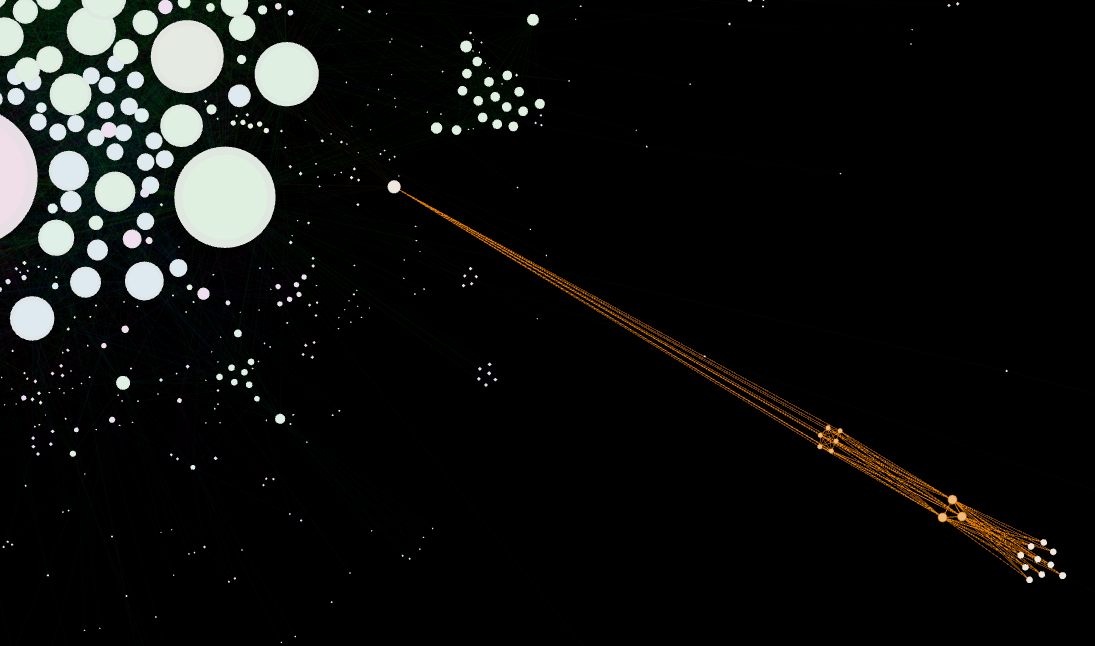
\includegraphics[width=60mm]{../figures/rt_net_photo}}
\subfloat[Boundary Spanner]{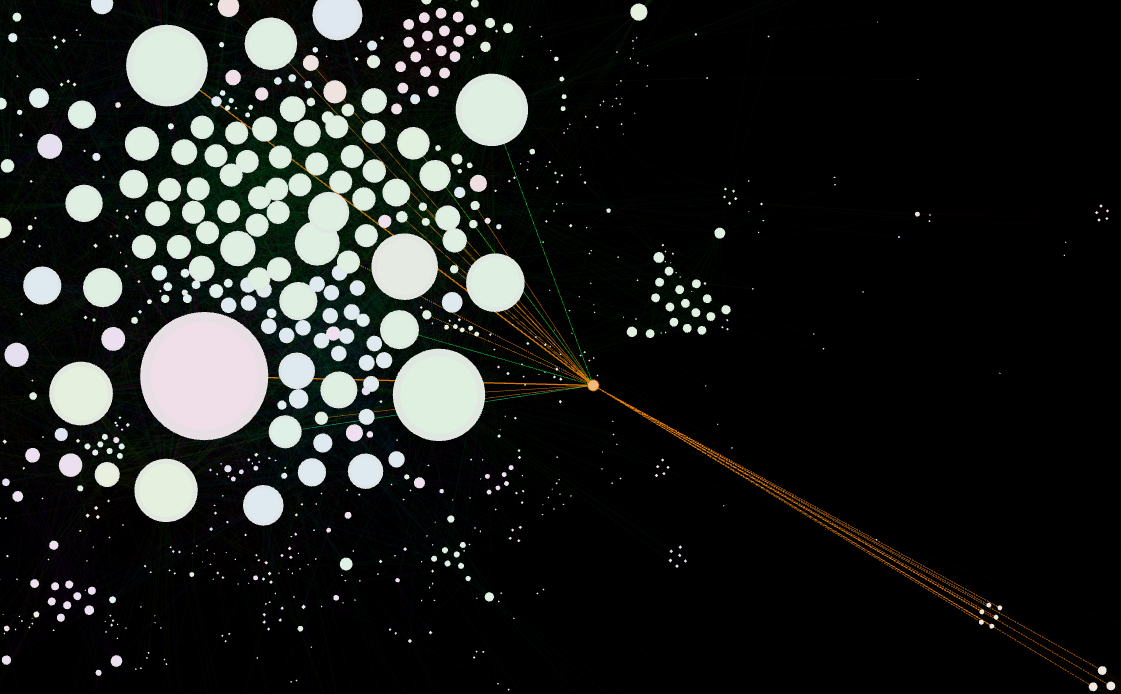
\includegraphics[width=60mm]{../figures/rt_net_photo_popular}}
\caption{Clusters of tweets representing sets of photos.}
\end{figure}

\section{Groups}

\section{Conclusion}

\bibliographystyle{llncs}
\bibliography{bibfile}

\end{document}
